\subsection{Introduction to Distributed Matrices}
\makesubcontentsslidessec


\begin{frame}
  \begin{block}{Distributed Matrices}\pause
  \begin{center}
  You can only get so far with one node\dots\\[.4cm]
    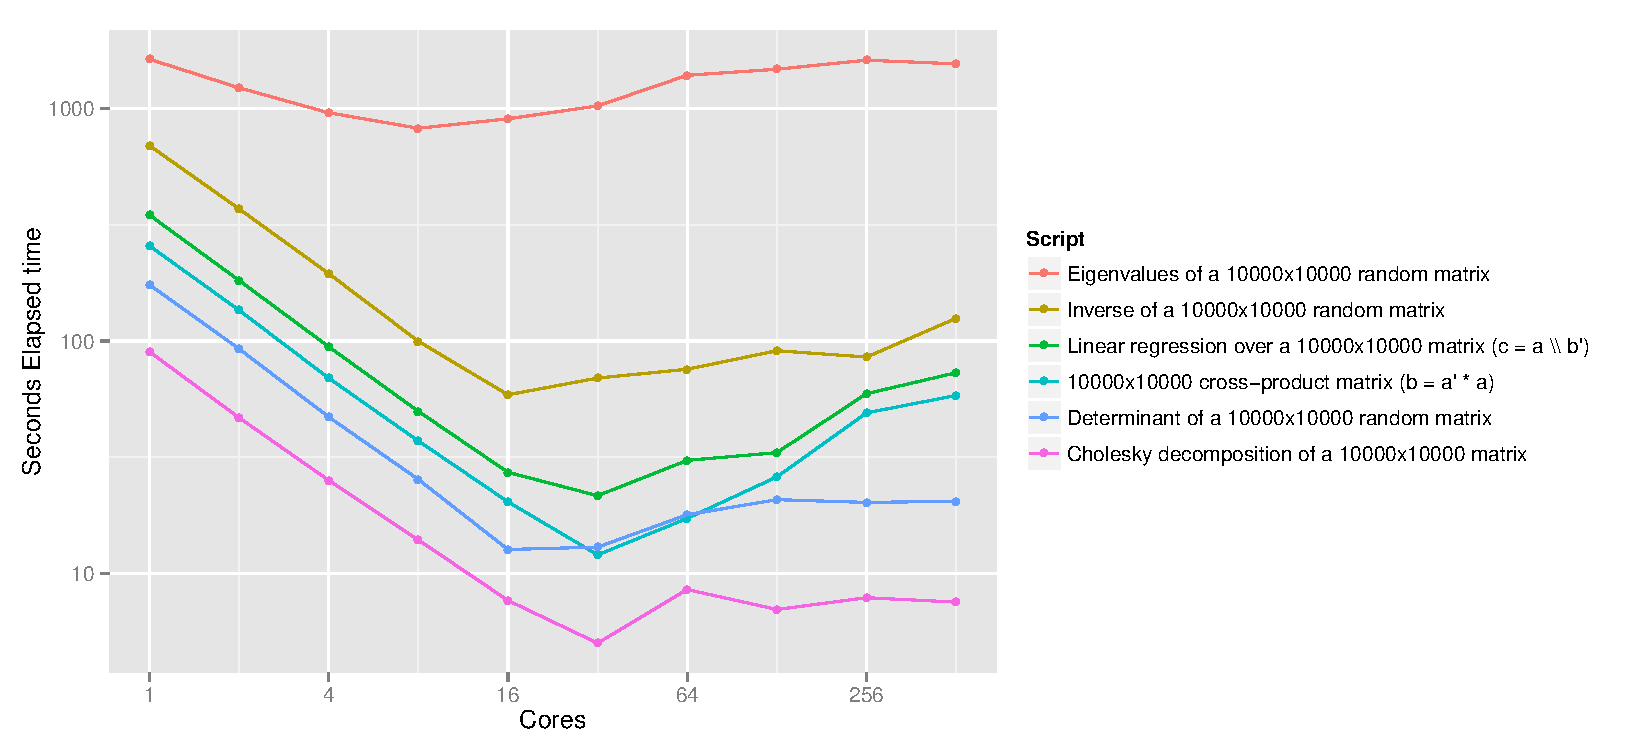
\includegraphics[width=.95\textwidth]{../common/pics/r_mkl_times}
    \\[.4cm]
    The solution is to distribute the data.
  \end{center}
  \end{block}
\end{frame}


% \begin{frame}[fragile]
%   \begin{block}{Distributed Matrices}\pause
%   High level OOP allows \emph{native} serial R syntax:
%   \begin{lstlisting}
% x <- x[-1, 2:5]
% x <- log(abs(x) + 1)
% xtx <- t(x) %*% x
% ans <- svd(solve(xtx))
%   \end{lstlisting}
%   \vspace{.4cm}
%   However\dots
%   \end{block}
% \end{frame}
% 
% 
% \begin{frame}
%   \begin{block}{Distributed Matrices}\pause
%   ddmatrix:
%     \begin{itemize}
%      \item \textbf{D}istributed \textbf{MAT}rix data structure.
%      \item No single processor should hold all of the data.
%      \item Block-cyclic matrix distributed across a 2-dimensional grid of processors.
%      \item Very robust, but confusing data structure.
%     \end{itemize}
%   \end{block}
% \end{frame}



\begin{frame}
\begin{block}{Distributed Matrices}
\begin{figure}[ht]
        \centering
        \begin{subfigure}[b]{0.3\textwidth}
                \centering
\includegraphics[height=5cm,width=\textwidth]%
{../common/pics/dmat/dmat_block}
                \caption{Row Block}
        \end{subfigure}
        \hspace{.1cm}
        \begin{subfigure}[b]{0.3\textwidth}
                \centering
                
\includegraphics[height=5cm,width=\textwidth]%
{../common/pics/dmat/dmat_cyclic}
                \caption{Row Cyclic}
        \end{subfigure}
        \hspace{.01cm}
        \begin{subfigure}[b]{0.3\textwidth}
                \centering
                
\includegraphics[height=5cm,width=\textwidth]%
{../common/pics/dmat/dmat_blockcyclic}
                \caption{Row-Block Cyclic}
        \end{subfigure}
        \caption{Matrix Distribution Schemes Onto a $4\times 1$
          Processor Grid}\label{fig:dmat1d}
\end{figure}
\end{block}
\end{frame}



\begin{frame}
\begin{block}{Distributed Matrices}
\begin{figure}[ht]
        \centering
        \begin{subfigure}[b]{0.3\textwidth}
                \centering
                
\includegraphics[height=5cm,width=\textwidth]%
{../common/pics/dmat/dmat_block2d}
                \caption{Block}
        \end{subfigure}%
        \hspace{.1cm}
        \begin{subfigure}[b]{0.3\textwidth}
                \centering
                
\includegraphics[height=5cm,width=\textwidth]%
{../common/pics/dmat/dmat_cyclic2d}
                \caption{Column-Block Row-Cyclic}
        \end{subfigure}
        \hspace{.01cm}
        \begin{subfigure}[b]{0.3\textwidth}
                \centering
                
\includegraphics[height=5cm,width=\textwidth]%
{../common/pics/dmat/dmat_blockcyclic2d}
                \caption{Block-Cyclic}
        \end{subfigure}
        \caption{Matrix Distribution Schemes Onto a $2\times 2$ Processor 
Grid}\label{fig:dmat2d}
\end{figure}
\end{block}
\end{frame}



\begin{frame}
\begin{block}{Processor Grid Shapes}
\begin{table}[ht]
        \centering
        \begin{subfigure}[b]{0.23\textwidth}
                \centering
              $\left[\begin{tabular}{l}
                  0 \\ 1 \\ 2 \\ 3 \\ 4 \\ 5
                \end{tabular}\right]^T$
                \caption{$1\times 6$}
        \end{subfigure}
        \begin{subfigure}[b]{0.23\textwidth}
                \centering
                $\left[\begin{tabular}{lll}
                  0 & 1 & 2\\
                  3 & 4 & 5
                \end{tabular}\right]$
                \caption{$2\times 3$}
        \end{subfigure}%
        \begin{subfigure}[b]{0.23\textwidth}
                \centering
              $\left[\begin{tabular}{ll}
                  0 & 1 \\
                  2 & 3\\
                  4 & 5
                \end{tabular}\right]$
                \caption{$3\times 2$}
        \end{subfigure}
        \begin{subfigure}[b]{0.23\textwidth}
                \centering
              $\left[\begin{tabular}{l}
                  0 \\ 1 \\ 2 \\ 3 \\ 4 \\ 5
                \end{tabular}\right]$
                \caption{$6\times 1$}
        \end{subfigure}
        \caption{Processor Grid Shapes with 6 Processors}\label{fig:gridshapes}
\end{table}
\end{block}
\end{frame}





\begin{frame}
  \begin{block}{The ddmatrix Class}\pause
  For \textbf{d}istributed \textbf{d}ense \textbf{matrix} objects, we use the 
special S4 class \code{ddmatrix}.

  \begin{align*}
  \hspace{.1cm}\text{\code{ddmatrix}}&=\begin{cases}
  $\textbf{Data}$ & $The local submatrix (an R matrix)$\\
  $\textbf{dim}$ & $Dimension of the global matrix$\\
  $\textbf{ldim}$ & $Dimension of the local submatrix$\\
  $\textbf{bldim}$ & $Dimension of the blocks$\\
  $\textbf{ICTXT}$ & $MPI Grid Context$
  \end{cases}
  \end{align*}

  \end{block}
\end{frame}


% \begin{frame}
%   \begin{block}{Distributed Matrices:  The Data Structure}\pause
%       Example:  an $9\times 9$ matrix is distributed with a ``block-cycling'' 
% factor of $2\times 2$ on a $2\times 2$ processor grid:
%       \begin{center}
%       \begin{minipage}{.45\textwidth}
%       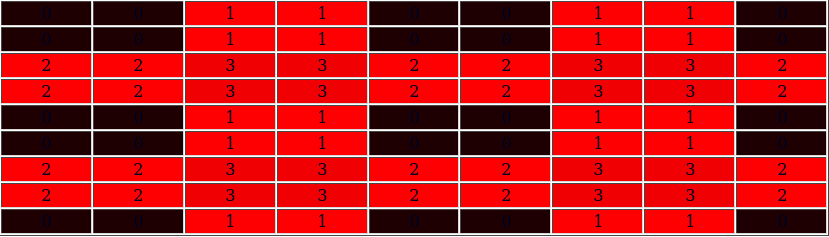
\includegraphics[width=5cm, height=4cm]{../common/pics/dmat/dmat_dist}  
%       \end{minipage}\hspace{.1cm}
%       \begin{minipage}{.45\textwidth}
%       \begin{center}
%       \begin{align*}
%         &=\begin{cases}
%         $\textbf{Data}$ & =\text{\code{matrix(\dots)}}\\
%         $\textbf{dim}$ & =\text{\code{c(9, 9)}}\\
%         $\textbf{ldim}$ & =\text{\code{c(\dots)}}\\
%         $\textbf{bldim}$ & =\text{\code{c(2, 2)}}\\
%         $\textbf{CTXT}$ & =0
%         \end{cases}
%         \end{align*}
%       \end{center}
%       \end{minipage}
%       \end{center}
%     {\small See \url{http://acts.nersc.gov/scalapack/hands-on/datadist.html}}
%   \end{block}
% \end{frame}



\begin{frame}
\begin{exampleblock}{Understanding \code{ddmatrix}: Global Matrix}
\begin{align*}
x &= \left[
      \begin{array}{lllllllll}
      x_{11} & x_{12} & x_{13} & x_{14} & x_{15} & x_{16} & x_{17} & x  _{18} & 
x_{19}\\
      x_{21} & x_{22} & x_{23} & x_{24} & x_{25} & x_{26} & x_{27} & x  _{28} & 
x_{29}\\
      x_{31} & x_{32} & x_{33} & x_{34} & x_{35} & x_{36} & x_{37} & x  _{38} & 
x_{39}\\
      x_{41} & x_{42} & x_{43} & x_{44} & x_{45} & x_{46} & x_{47} & x  _{48} & 
x_{49}\\
      x_{51} & x_{52} & x_{53} & x_{54} & x_{55} & x_{56} & x_{57} & x  _{58} & 
x_{59}\\
      x_{61} & x_{62} & x_{63} & x_{64} & x_{65} & x_{66} & x_{67} & x  _{68} & 
x_{69}\\
      x_{71} & x_{72} & x_{73} & x_{74} & x_{75} & x_{76} & x_{77} & x  _{78} & 
x_{79}\\
      x_{81} & x_{82} & x_{83} & x_{84} & x_{85} & x_{86} & x_{87} & x  _{88} & 
x_{89}\\
      x_{91} & x_{92} & x_{93} & x_{94} & x_{95} & x_{96} & x_{97} & x  _{98} & 
x_{99}
      \end{array}
\right]_{9\times 9}
\end{align*}
\end{exampleblock}
\end{frame}



\begin{frame}
\begin{exampleblock}{\code{ddmatrix}:  Row Block}
\begin{align*}
x &= \left[
      \begin{array}{lllllllll}
      \color{g11}x_{11} & \color{g11}x_{12} & \color{g11}x_{13} & 
\color{g11}x_{14} & \color{g11}x_{15} & \color{g11}x_{16} & \color{g11}x_{17} & 
\color{g11}x_{18} & \color{g11}x_{19}\\
      \color{g11}x_{21} & \color{g11}x_{22} & \color{g11}x_{23} & 
\color{g11}x_{24} & \color{g11}x_{25} & \color{g11}x_{26} & \color{g11}x_{27} & 
\color{g11}x_{28} & \color{g11}x_{29}\\
      \color{g11}x_{31} & \color{g11}x_{32} & \color{g11}x_{33} & 
\color{g11}x_{34} & \color{g11}x_{35} & \color{g11}x_{36} & \color{g11}x_{37} & 
\color{g11}x_{38} & \color{g11}x_{39}\\\hline
      \color{g12}x_{41} & \color{g12}x_{42} & \color{g12}x_{43} & 
\color{g12}x_{44} & \color{g12}x_{45} & \color{g12}x_{46} & \color{g12}x_{47} & 
\color{g12}x_{48} & \color{g12}x_{49}\\
      \color{g12}x_{51} & \color{g12}x_{52} & \color{g12}x_{53} & 
\color{g12}x_{54} & \color{g12}x_{55} & \color{g12}x_{56} & \color{g12}x_{57} & 
\color{g12}x_{58} & \color{g12}x_{59}\\
      \color{g12}x_{61} & \color{g12}x_{62} & \color{g12}x_{63} & 
\color{g12}x_{64} & \color{g12}x_{65} & \color{g12}x_{66} & \color{g12}x_{67} & 
\color{g12}x_{68} & \color{g12}x_{69}\\\hline
      \color{g13}x_{71} & \color{g13}x_{72} & \color{g13}x_{73} & 
\color{g13}x_{74} & \color{g13}x_{75} & \color{g13}x_{76} & \color{g13}x_{77} & 
\color{g13}x_{78} & \color{g13}x_{79}\\
      \color{g13}x_{81} & \color{g13}x_{82} & \color{g13}x_{83} & 
\color{g13}x_{84} & \color{g13}x_{85} & \color{g13}x_{86} & \color{g13}x_{87} & 
\color{g13}x_{88} & \color{g13}x_{89}\\
      \color{g13}x_{91} & \color{g13}x_{92} & \color{g13}x_{93} & 
\color{g13}x_{94} & \color{g13}x_{95} & \color{g13}x_{96} & \color{g13}x_{97} & 
\color{g13}x_{98} & \color{g13}x_{99}\\
      \end{array}
\right]_{9\times 9}
\end{align*}
\vspace{-.6cm}
\begin{align*}
\text{Processor grid = }\left|
      \begin{array}{l}
      \color{g11}0 \\
      \color{g12}1 \\
      \color{g13}2 \\
      \color{g21}3
      \end{array}
\right| &
% = \left|
%      \begin{tabular}{l}
%      \color{g11}(0,0) \\
%      \color{g12}(1,0) \\
%      \color{g13}(2,0) \\
%      \color{g21}(3,0) 
%      \end{tabular}
%\right|
\end{align*}
\end{exampleblock}
\end{frame}





\begin{frame}
\begin{exampleblock}{\code{ddmatrix}: Row-Column Block}
\begin{align*}
x &= \left[
      \begin{array}{lllll|llll}
      \color{g11}x_{11} & \color{g11}x_{12} & \color{g11}x_{13} & 
\color{g11}x_{14} & \color{g11}x_{15} & \color{g12}x_{16} & \color{g12}x_{17} & 
\color{g12}x_{18} & \color{g12}x_{19}\\
      \color{g11}x_{21} & \color{g11}x_{22} & \color{g11}x_{23} & 
\color{g11}x_{24} & \color{g11}x_{25} & \color{g12}x_{26} & \color{g12}x_{27} & 
\color{g12}x_{28} & \color{g12}x_{29}\\
      \color{g11}x_{31} & \color{g11}x_{32} & \color{g11}x_{33} & 
\color{g11}x_{34} & \color{g11}x_{35} & \color{g12}x_{36} & \color{g12}x_{37} & 
\color{g12}x_{38} & \color{g12}x_{39}\\
      \color{g11}x_{41} & \color{g11}x_{42} & \color{g11}x_{43} & 
\color{g11}x_{44} & \color{g11}x_{45} & \color{g12}x_{46} & \color{g12}x_{47} & 
\color{g12}x_{48} & \color{g12}x_{49}\\
      \color{g11}x_{51} & \color{g11}x_{52} & \color{g11}x_{53} & 
\color{g11}x_{54} & \color{g11}x_{55} & \color{g12}x_{56} & \color{g12}x_{57} & 
\color{g12}x_{58} & \color{g12}x_{59}\\\hline
      \color{g13}x_{61} & \color{g13}x_{62} & \color{g13}x_{63} & 
\color{g13}x_{64} & \color{g13}x_{65} & \color{g21}x_{66} & \color{g21}x_{67} & 
\color{g21}x_{68} & \color{g21}x_{69}\\
      \color{g13}x_{71} & \color{g13}x_{72} & \color{g13}x_{73} & 
\color{g13}x_{74} & \color{g13}x_{75} & \color{g21}x_{76} & \color{g21}x_{77} & 
\color{g21}x_{78} & \color{g21}x_{79}\\
      \color{g13}x_{81} & \color{g13}x_{82} & \color{g13}x_{83} & 
\color{g13}x_{84} & \color{g13}x_{85} & \color{g21}x_{86} & \color{g21}x_{87} & 
\color{g21}x_{88} & \color{g21}x_{89}\\
      \color{g13}x_{91} & \color{g13}x_{92} & \color{g13}x_{93} & 
\color{g13}x_{94} & \color{g13}x_{95} & \color{g21}x_{96} & \color{g21}x_{97} & 
\color{g21}x_{98} & \color{g21}x_{99}\\
      \end{array}
\right]_{9\times 9}
\end{align*}
\begin{align*}
\text{Processor grid = }\left|
      \begin{array}{ll}
      \color{g11}0 & \color{g12}1 \\
      \color{g13}2 & \color{g21}3
      \end{array}
\right| &= 
\left|
      \begin{tabular}{lll}
      \color{g11}(0,0) & \color{g12}(0,1) \\
      \color{g13}(1,0) & \color{g21}(1,1) 
      \end{tabular}
\right|
\end{align*}
\end{exampleblock}
\end{frame}



\begin{frame}
\begin{exampleblock}{\code{ddmatrix}: Row Cyclic}
\begin{align*}
x &= \left[
      \begin{array}{lllllllll}
      \color{g11}x_{11} & \color{g11}x_{12} & \color{g11}x_{13} & 
\color{g11}x_{14} & \color{g11}x_{15} & \color{g11}x_{16} & \color{g11}x_{17} & 
\color{g11}x_{18} & \color{g11}x_{19}\\\hline
      \color{g12}x_{21} & \color{g12}x_{22} & \color{g12}x_{23} & 
\color{g12}x_{24} & \color{g12}x_{25} & \color{g12}x_{26} & \color{g12}x_{27} & 
\color{g12}x_{28} & \color{g12}x_{29}\\\hline
      \color{g13}x_{31} & \color{g13}x_{32} & \color{g13}x_{33} & 
\color{g13}x_{34} & \color{g13}x_{35} & \color{g13}x_{36} & \color{g13}x_{37} & 
\color{g13}x_{38} & \color{g13}x_{39}\\\hline
      \color{g21}x_{41} & \color{g21}x_{42} & \color{g21}x_{43} & 
\color{g21}x_{44} & \color{g21}x_{45} & \color{g21}x_{46} & \color{g21}x_{47} & 
\color{g21}x_{48} & \color{g21}x_{49}\\\hline
      \color{g11}x_{51} & \color{g11}x_{52} & \color{g11}x_{53} & 
\color{g11}x_{54} & \color{g11}x_{55} & \color{g11}x_{56} & \color{g11}x_{57} & 
\color{g11}x_{58} & \color{g11}x_{59}\\\hline
      \color{g12}x_{61} & \color{g12}x_{62} & \color{g12}x_{63} & 
\color{g12}x_{64} & \color{g12}x_{65} & \color{g12}x_{66} & \color{g12}x_{67} & 
\color{g12}x_{68} & \color{g12}x_{69}\\\hline
      \color{g13}x_{71} & \color{g13}x_{72} & \color{g13}x_{73} & 
\color{g13}x_{74} & \color{g13}x_{75} & \color{g13}x_{76} & \color{g13}x_{77} & 
\color{g13}x_{78} & \color{g13}x_{79}\\\hline
      \color{g21}x_{81} & \color{g21}x_{82} & \color{g21}x_{83} & 
\color{g21}x_{84} & \color{g21}x_{85} & \color{g21}x_{86} & \color{g21}x_{87} & 
\color{g21}x_{88} & \color{g21}x_{89}\\\hline
      \color{g11}x_{91} & \color{g11}x_{92} & \color{g11}x_{93} & 
\color{g11}x_{94} & \color{g11}x_{95} & \color{g11}x_{96} & \color{g11}x_{97} & 
\color{g11}x_{98} & \color{g11}x_{99}\\
      \end{array}
\right]_{9\times 9}
\end{align*}
\vspace{-.6cm}
\begin{align*}
\text{Processor grid = }\left|
      \begin{array}{l}
      \color{g11}0 \\
      \color{g12}1 \\
      \color{g13}2 \\
      \color{g21}3
      \end{array}
\right| &
%= \left|
%      \begin{tabular}{lll}
%      \color{g11}(0,0) \\
%      \color{g12}(1,0) \\
%      \color{g13}(2,0) \\
%      \color{g21}(3,0) 
%      \end{tabular}
%\right|
\end{align*}
\end{exampleblock}
\end{frame}



\begin{frame}
\begin{exampleblock}{\code{ddmatrix}: Row-Cyclic Column-Block}
\begin{align*}
x &= \left[
      \begin{array}{lllll|llll}
      \color{g11}x_{11} & \color{g11}x_{12} & \color{g11}x_{13} & 
\color{g11}x_{14} & \color{g11}x_{15} & \color{g12}x_{16} & \color{g12}x_{17} & 
\color{g12}x_{18} & \color{g12}x_{19}\\\hline
      \color{g13}x_{21} & \color{g13}x_{22} & \color{g13}x_{23} & 
\color{g13}x_{24} & \color{g13}x_{25} & \color{g21}x_{26} & \color{g21}x_{27} & 
\color{g21}x_{28} & \color{g21}x_{29}\\\hline
      \color{g11}x_{31} & \color{g11}x_{32} & \color{g11}x_{33} & 
\color{g11}x_{34} & \color{g11}x_{35} & \color{g12}x_{36} & \color{g12}x_{37} & 
\color{g12}x_{38} & \color{g12}x_{39}\\\hline
      \color{g13}x_{41} & \color{g13}x_{42} & \color{g13}x_{43} & 
\color{g13}x_{44} & \color{g13}x_{45} & \color{g21}x_{46} & \color{g21}x_{47} & 
\color{g21}x_{48} & \color{g21}x_{49}\\\hline
      \color{g11}x_{51} & \color{g11}x_{52} & \color{g11}x_{53} & 
\color{g11}x_{54} & \color{g11}x_{55} & \color{g12}x_{56} & \color{g12}x_{57} & 
\color{g12}x_{58} & \color{g12}x_{59}\\\hline
      \color{g13}x_{61} & \color{g13}x_{62} & \color{g13}x_{63} & 
\color{g13}x_{64} & \color{g13}x_{65} & \color{g21}x_{66} & \color{g21}x_{67} & 
\color{g21}x_{68} & \color{g21}x_{69}\\\hline
      \color{g11}x_{71} & \color{g11}x_{72} & \color{g11}x_{73} & 
\color{g11}x_{74} & \color{g11}x_{75} & \color{g12}x_{76} & \color{g12}x_{77} & 
\color{g12}x_{78} & \color{g12}x_{79}\\\hline
      \color{g13}x_{81} & \color{g13}x_{82} & \color{g13}x_{83} & 
\color{g13}x_{84} & \color{g13}x_{85} & \color{g21}x_{86} & \color{g21}x_{87} & 
\color{g21}x_{88} & \color{g21}x_{89}\\\hline
      \color{g11}x_{91} & \color{g11}x_{92} & \color{g11}x_{93} & 
\color{g11}x_{94} & \color{g11}x_{95} & \color{g12}x_{96} & \color{g12}x_{97} & 
\color{g12}x_{98} & \color{g12}x_{99}\\
      \end{array}
\right]_{9\times 9}
\end{align*}
\begin{align*}
\text{Processor grid = }\left|
      \begin{array}{ll}
      \color{g11}0 & \color{g12}1 \\
      \color{g13}2 & \color{g21}3
      \end{array}
\right| &= 
\left|
      \begin{tabular}{lll}
      \color{g11}(0,0) & \color{g12}(0,1) \\
      \color{g13}(1,0) & \color{g21}(1,1) 
      \end{tabular}
\right|
\end{align*}
\end{exampleblock}
\end{frame}




\begin{frame}[shrink]
\begin{exampleblock}{\code{ddmatrix}: Block-Cyclic}
\begin{align*}
x &= \left[
      \begin{array}{ll|ll|ll|ll|l}
      \color{g11}x_{11} & \color{g11}x_{12} & \color{g12}x_{13} & 
\color{g12}x_{14} & 
\color{g11}x_{15} & \color{g11}x_{16} & \color{g12}x_{17} & \color{g12}x_{18} & 
\color{g11}x_{19}\\
      \color{g11}x_{21} & \color{g11}x_{22} & \color{g12}x_{23} & 
\color{g12}x_{24} & 
\color{g11}x_{25} & \color{g11}x_{26} & \color{g12}x_{27} & \color{g12}x_{28} & 
\color{g11}x_{29}\\\hline
      \color{g13}x_{31} & \color{g13}x_{32} & \color{g21}x_{33} & 
\color{g21}x_{34} & 
\color{g13}x_{35} & \color{g13}x_{36} & \color{g21}x_{37} & \color{g21}x_{38} & 
\color{g13}x_{39}\\
      \color{g13}x_{41} & \color{g13}x_{42} & \color{g21}x_{43} & 
\color{g21}x_{44} & 
\color{g13}x_{45} & \color{g13}x_{46} & \color{g21}x_{47} & \color{g21}x_{48} & 
\color{g13}x_{49}\\\hline
      \color{g11}x_{51} & \color{g11}x_{52} & \color{g12}x_{53} & 
\color{g12}x_{54} & 
\color{g11}x_{55} & \color{g11}x_{56} & \color{g12}x_{57} & \color{g12}x_{58} & 
\color{g11}x_{59}\\
      \color{g11}x_{61} & \color{g11}x_{62} & \color{g12}x_{63} & 
\color{g12}x_{64} & 
\color{g11}x_{65} & \color{g11}x_{66} & \color{g12}x_{67} & \color{g12}x_{68} & 
\color{g11}x_{69}\\\hline
      \color{g13}x_{71} & \color{g13}x_{72} & \color{g21}x_{73} & 
\color{g21}x_{74} & 
\color{g13}x_{75} & \color{g13}x_{76} & \color{g21}x_{77} & \color{g21}x_{78} & 
\color{g13}x_{79}\\
      \color{g13}x_{81} & \color{g13}x_{82} & \color{g21}x_{83} & 
\color{g21}x_{84} & 
\color{g13}x_{85} & \color{g13}x_{86} & \color{g21}x_{87} & \color{g21}x_{88} & 
\color{g13}x_{89}\\\hline
      \color{g11}x_{91} & \color{g11}x_{92} & \color{g12}x_{93} & 
\color{g12}x_{94} & 
\color{g11}x_{95} & \color{g11}x_{96} & \color{g12}x_{97} & \color{g12}x_{98} & 
\color{g11}x_{99}\\
      \end{array}
\right]_{9\times 9}
\end{align*}
\begin{align*}
\text{Processor grid = }\left|
      \begin{array}{ll}
      \color{g11}0 & \color{g12}1 \\
      \color{g13}2 & \color{g21}3
      \end{array}
\right| &= 
\left|
      \begin{tabular}{lll}
      \color{g11}(0,0) & \color{g12}(0,1) \\
      \color{g13}(1,0) & \color{g21}(1,1) 
      \end{tabular}
\right|
\end{align*}
\end{exampleblock}
\end{frame}


